\documentclass[12pt, letterpaper]{article}

\usepackage{color} %% Allows text to be typeset in color.

%% These allow Me to add Images to the Book.
\usepackage{graphicx}
\graphicspath{ {images/} }

%% Enables hyperlinks.
\usepackage{hyperref}

%% Makes BigO easier.
\newcommand{\bigO}{\mathcal{O}}
\newcommand{\bigOmega}{\Omega}
\newcommand{\bigTheta}{\Theta}

%%
\oddsidemargin0cm
\evensidemargin0cm
\topmargin-2cm     % These lines increase the amount of usable space and save trees.
\textwidth16.5cm
\textheight23.5cm  

%%\setcounter{tocdepth}{4} %% set the table of contents detail depth.

%% Types of organizational sections.s
%%\part{}
%%\chapter{}
%%\section{}
%%\subsection{}
%%\subsubsection{}
%%\paragraph{}
%%\subparagraph{}

\begin{document}

\title{\color{blue}Hump Yard Rules v1.2}
\author{Written by Bryce Summers \texttt(BryceSummers.com)}
\date{\color{red}Last Updated: \today}
\maketitle

\tableofcontents 

\section{Overview}

Hump Yard is a game about efficiently managing a rail classification yard. Players procure train cars and track, build networks, and engage in strategic trading.

\newpage
\section{Components}

Hump Yard comes with 4 of each of the following \textit{normal} Track tiles:


\includegraphics[width=0.20\textwidth]{Track_0.png}

\includegraphics[width=0.20\textwidth]{Track_3.png}
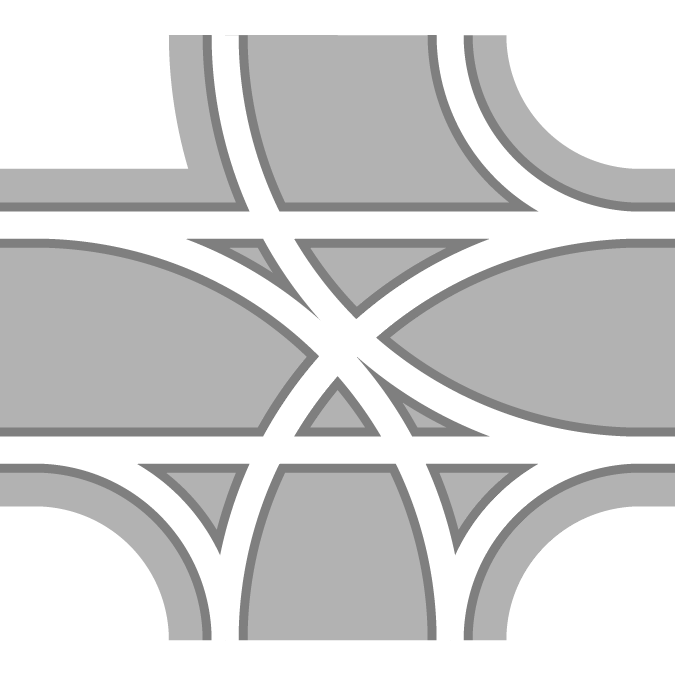
\includegraphics[width=0.20\textwidth]{Track_10.png}

\includegraphics[width=0.20\textwidth]{Track_22.png}

\includegraphics[width=0.20\textwidth]{Track_25.png}
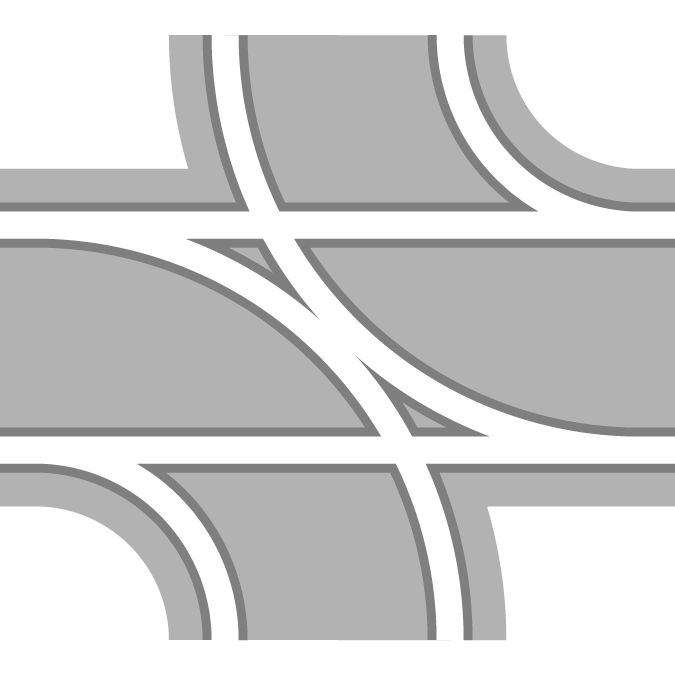
\includegraphics[width=0.20\textwidth]{Track_26.png}

\includegraphics[width=0.20\textwidth]{Track_32.png}

\includegraphics[width=0.20\textwidth]{Track_35.png}
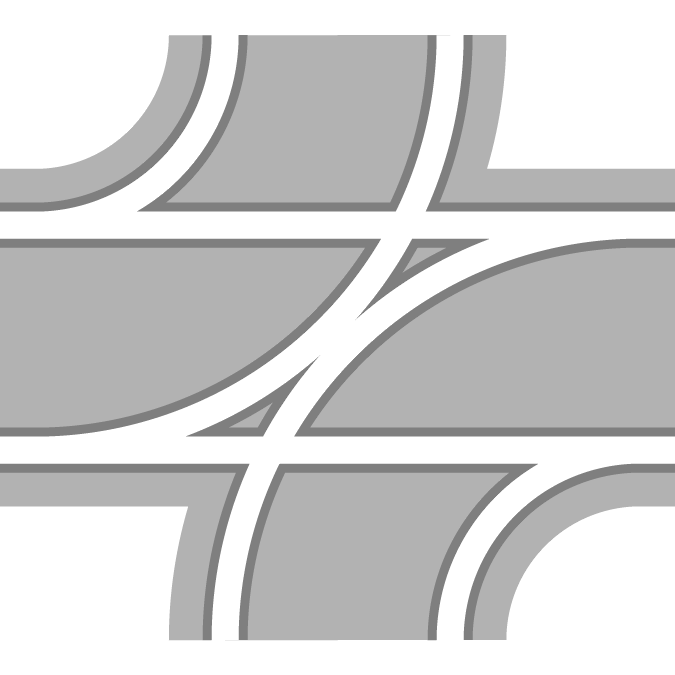
\includegraphics[width=0.20\textwidth]{Track_38.png}

\includegraphics[width=0.20\textwidth]{Track_39.png}

\includegraphics[width=0.20\textwidth]{Track_40.png}

\includegraphics[width=0.20\textwidth]{Track_41.png}

\includegraphics[width=0.20\textwidth]{Track_43.png}

\includegraphics[width=0.20\textwidth]{Track_44.png}

\includegraphics[width=0.20\textwidth]{Track_45.png}

\includegraphics[width=0.20\textwidth]{Track_55.png}

\includegraphics[width=0.20\textwidth]{Track_57.png}
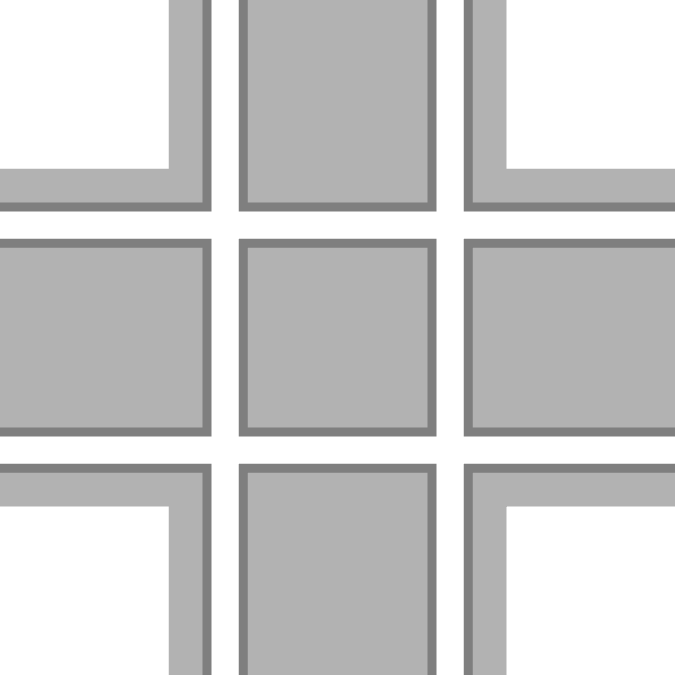
\includegraphics[width=0.20\textwidth]{Track_60.png}
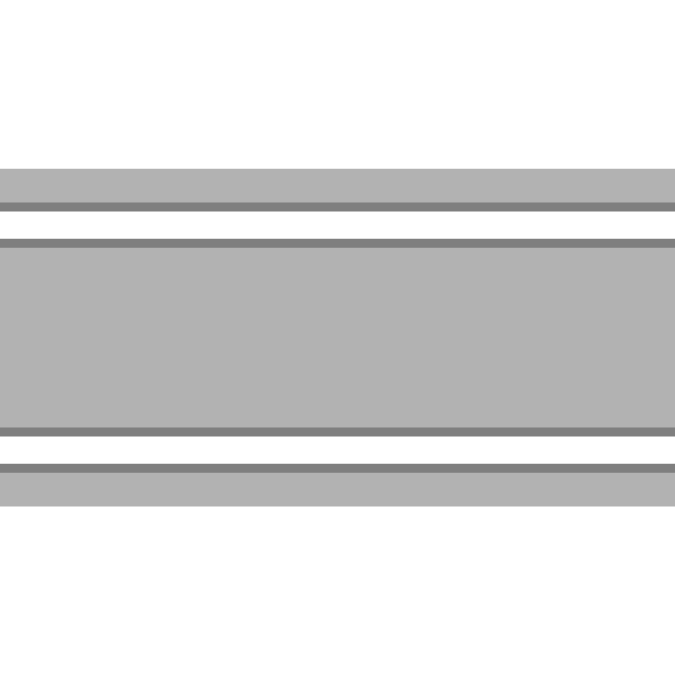
\includegraphics[width=0.20\textwidth]{Track_62.png}
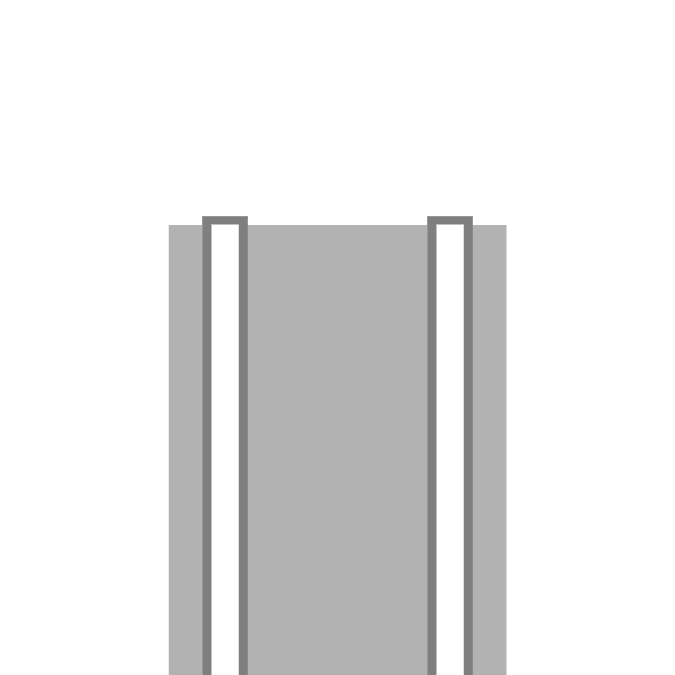
\includegraphics[width=0.20\textwidth]{Track_end.png}

5 of each of the following colored track headings:

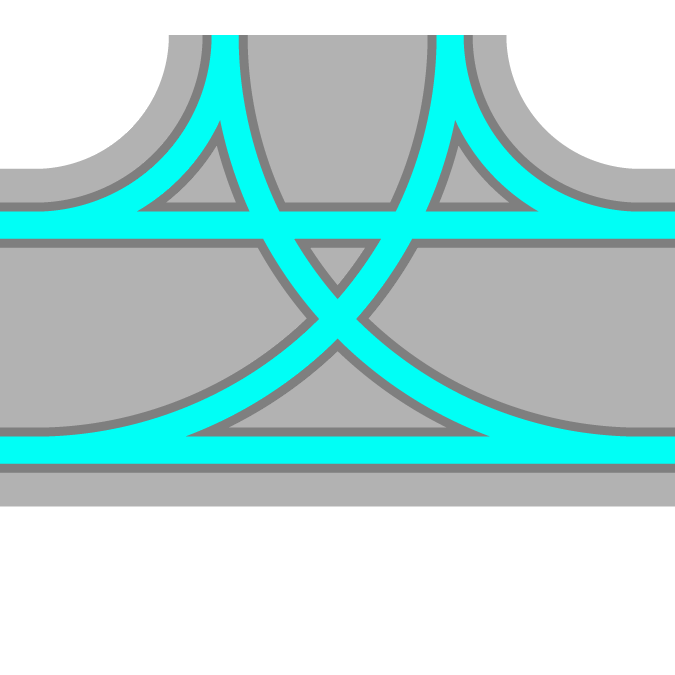
\includegraphics[width=0.20\textwidth]{BlueHeading.png}
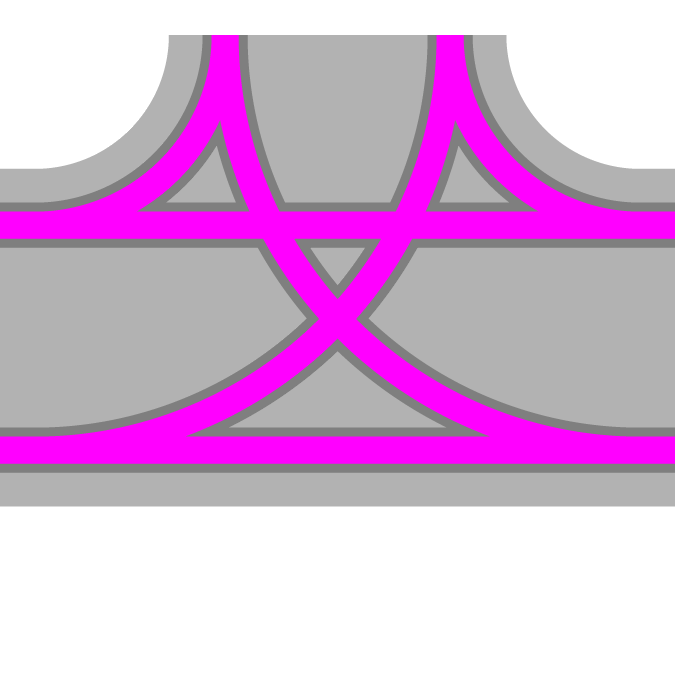
\includegraphics[width=0.20\textwidth]{PurpleHeading.png}
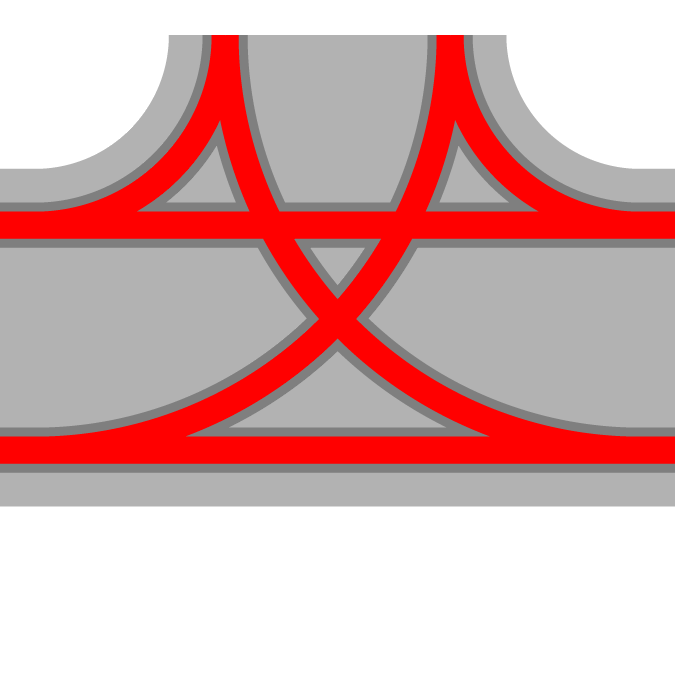
\includegraphics[width=0.20\textwidth]{RedHeading.png}
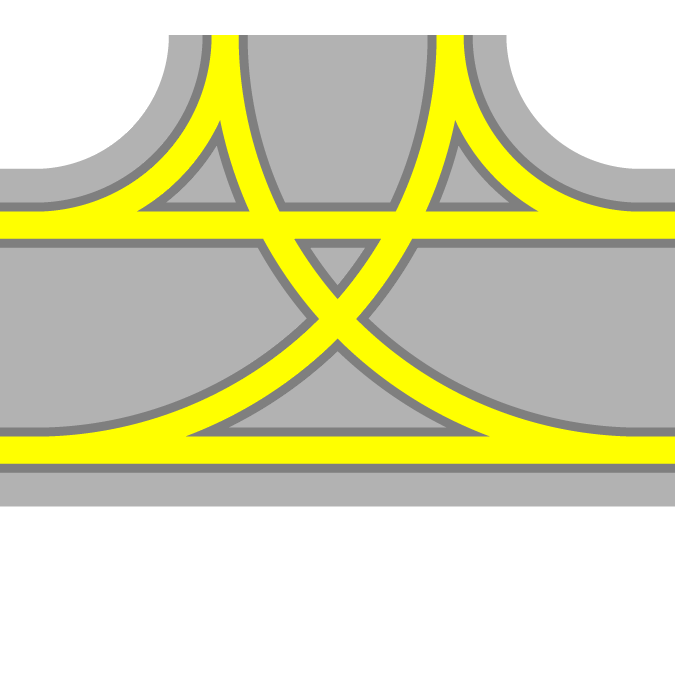
\includegraphics[width=0.20\textwidth]{YellowHeading.png}

8 Sources and 8 Sinks.

\includegraphics[width=0.25\textwidth]{Source.png} $\times 8$

\includegraphics[width=0.25\textwidth]{Sink.png} $\times 8$


\section{Game Play Regions}

\subsection{Track Market}
The track market is a region that will be used to store pieces of track that are currently being sold. Every turn players will bid for the right to purchase specific pieces of track. All players will receive one piece of track from the track marcket every turn.

\subsection{Train Contract Market}

The Train Contract Market is a region that will be used to store contracts that players may bid for. Contracts consist of sets of train cars that may be sold to a buyer. Players wish to obtain

\subsection{Train Car Market}

The Train Car Market is used to store train cars that are currently for sale. Cars are won by bidding and the minnimum bid of each car decreases over time.

\subsection{Player Yards}

Each Player has a yard area where they will build their yard and store and shunt train cars.

\subsection{Generating a Contract}

\subsection{Generating Rolling Stock}

\subsection{Shunting}

\newpage

\section{Rules of Play}

\subsection{Setup}

Every players sets up their yard as follows with 5 of their collored heading tracks sandwitched by a source and a sink:


\includegraphics[width=0.10\textwidth]{Source.png}
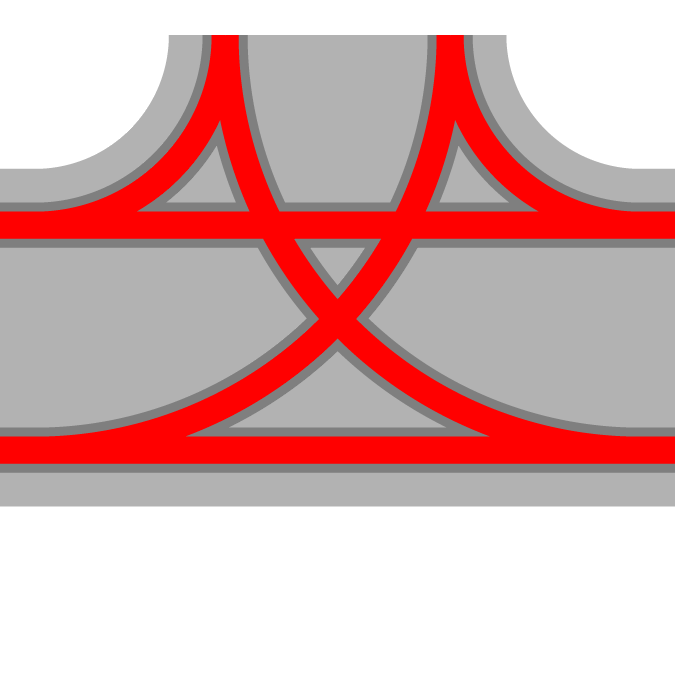
\includegraphics[width=0.10\textwidth]{RedHeading.png}
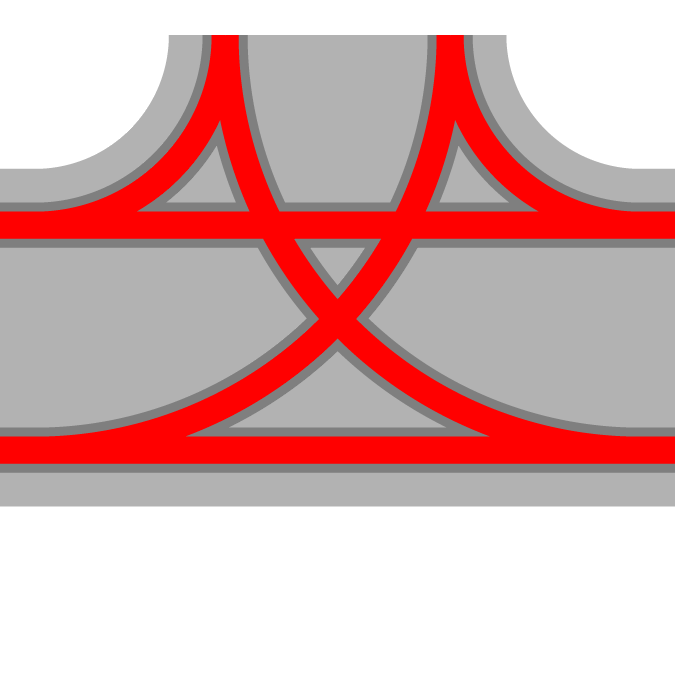
\includegraphics[width=0.10\textwidth]{RedHeading.png}
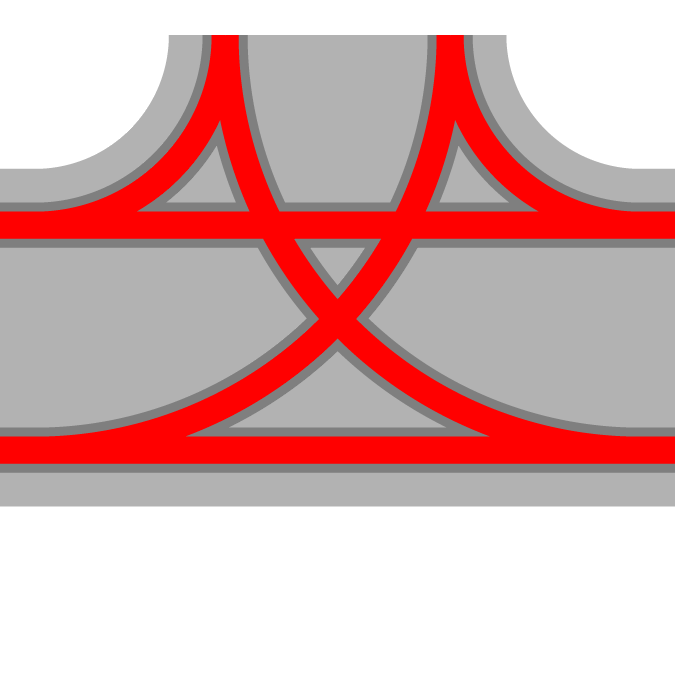
\includegraphics[width=0.10\textwidth]{RedHeading.png}
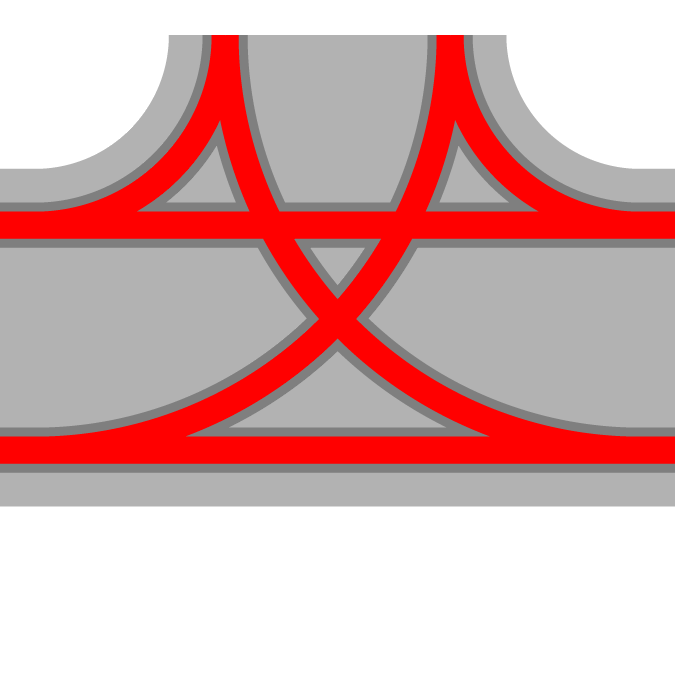
\includegraphics[width=0.10\textwidth]{RedHeading.png}
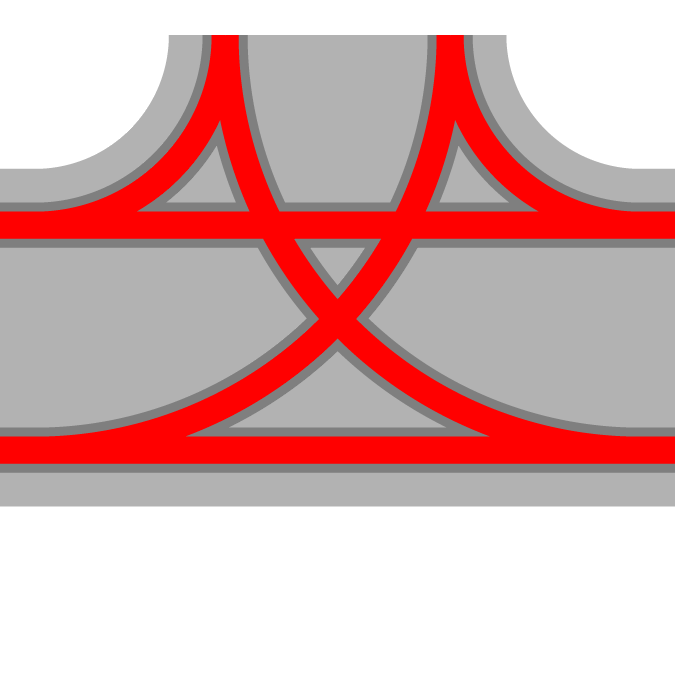
\includegraphics[width=0.10\textwidth]{RedHeading.png}

\includegraphics[width=0.10\textwidth]{Sink.png}

It is perfectly fine to have the headings point downwards if desired.
\begin{itemize}
\item Let $P$ be the number of players.
\item Place all of the Normal track pieces facedown in a stack. Take the first $P$ of these tiles, flip them face up and use them to start the track piece market.
\item Generate $P-1$ contracts and use them to start the Contract market.
\end{itemize}

\subsection{Turns}

Each turn consists of the following phases.

\subsubsection{Phase1 : Track Auction}

Maximum bid wins. Each player must buy exactly 1 piece of track each turn. Naturally, players that have bought track pieces may not engage in any other auctions that turn. Players are prohibited from bidding more money than they have on hand.

At the end of the auction, lay 1 new random track piece in the track market for every player in the game.

\subsubsection{Phase2 : Contract Auction}

Minimum bid wins the contract. Players may only have 1 contract active at a time and can only deactivate contracts by fullfilling them.
Naturally, players with active contracts may not take part in the bidding of any new contracts.

Everytime a contract is purchased, generate a new contract and place it in the contract market.

\subsubsection{Phase3 : Rolling Stock Auction}

Maximum bid wins. Players may buy as many or few pieces of rolling stock as they desire and can afford.

At the end of the auction, generate $Y$ new pieces of rolling stock.

\subsubsection{Phase 3: Trading, selling, and Shunting}

Players may pay $X$ to shunt a set of cars with one end accessible by the source or sink. Players may move cars to each other's yards by moving the cars to the sink, as long as the players have agreed to a trade agreement involving the amount of money that will change hands as compensation for the action.

In a similar way, players may shunt cars to the sink to fullfill contracts that have won and collect money from the bank.

Players may trade 3 cars to the bank for 1 car of any color.

\subsection{End of Game and Winning}
The game \textbf{ends} after 20 Turns have elapsed, which is when everyone will have a full yard with a piece of track in every square.

The player with the most money \textbf{wins} the game. If two players are tied, then the player with the most cars in their yard wins.


\subsection{New Turns}

\begin{itemize}
\item Players begin with the default yard and a 5 car contract.
\item Players take turns buying track pieces untill nobody wants one. Track pieces cost 1 coin.
\item Players may receive a random car for 2 coins. Players may move cars for 1 coin.
\item Players may make trades by spending coins to move their cars out of their yards and sending trains to other players.
\item Players may sell train cars to the bank for 1 coin.
\item Players may receive the first random car for free every turn.
\item Players may not leave any cars on their track headings between turns.
\item Players may satisfy contracts for 20 coins.
\item The Game ends when a player has a full 20 pieces of track in their yard.
\end{itemize}

\subsection{New Turns}

\begin{itemize}
\item Build the yard at the beginning of the game.
\item Buying cars.
\item Cars may only be used to fullfill contracts and sold to other players, they may not be ditched.
\end{itemize}

%% Signals that the document has ended.
\end{document}